\section{Introduction}
\label{sec:intro}

% Language models in the low-billions parameter range are increasingly fine-tuned with parameter-efficient adapters~\citep{hu2021lora, dettmers2023qlora}, where a fixed compute budget must absorb a stream of new tasks while reducing catastrophic forgetting. 

While context-augmented generation and external memory buffers effectively sustain short-term context in large language models, their high memory and inference latency overheads hinder real-time deployment on edge devices. For small-scale models, converting ephemeral context into long-term parameteric memory via supervised fine-tuning (SFT) is a compelling alternative; however, sequentially updating these parameters inevitably triggers catastrophic forgetting~\citep{hu2021lora, dettmers2023qlora}.
Continual learning for LoRA adapters updates only a chosen subset of parameters, and gradient attribution is the common rule for choosing it: a backward pass over held-out calibration data scores each parameter, and the highest-scoring ones are updated. Choosing the subset uniformly at random costs nothing instead, so whether the attribution pass earns its cost has a direct engineering answer.

% The question is harder to settle than it looks, because s
Standard zero-initialized LoRA introduces a confound. With $B = 0$ at initialization, $\partial \mathcal{L}/\partial A = 0$, so gradient attribution assigns zero importance to every \texttt{lora\_A} parameter and a gradient mask selects only from \texttt{lora\_B}, while the usual random baseline draws from both factors together. Any comparison that does not match the two pools therefore mixes the selection criterion with the parameter pool; the closest prior work, Attribution-Guided CL~\citep{liu2026attributionguided}, uses gradient attribution as a continual-learning mask on LLMs without matching the pool.

We separate the two by restricting both arms to the same pool and parameter count. On Qwen2.5-3B with rank-16 LoRA over a five-task sequence we compare a uniformly random mask on \texttt{lora\_B} (Random-B) against a gradient mask renormalised to the same 10\% of \texttt{lora\_B} (Grad-B), so both train exactly the same parameters and differ only in how those parameters are chosen. Across seven seeds the random mask achieves the lower loss-based backward transfer, and the gap holds in every seed (Table~\ref{tab:d1}, Figure~\ref{fig:headline}). The aggregate gap is concentrated on the medical task, with code and math moving in the same direction
and legal showing no reliable difference,
 a pattern consistent with a stability--plasticity trade-off: the random mask fits each task less well on its own diagonal yet retains earlier tasks better. 
 % All reported forgetting metrics are loss-based BWT. All headline comparisons are within-run.
 Above all, this work makes two key contributions:

\begin{figure}[t]
\centering
\begin{minipage}[b]{0.8\textwidth}
\centering
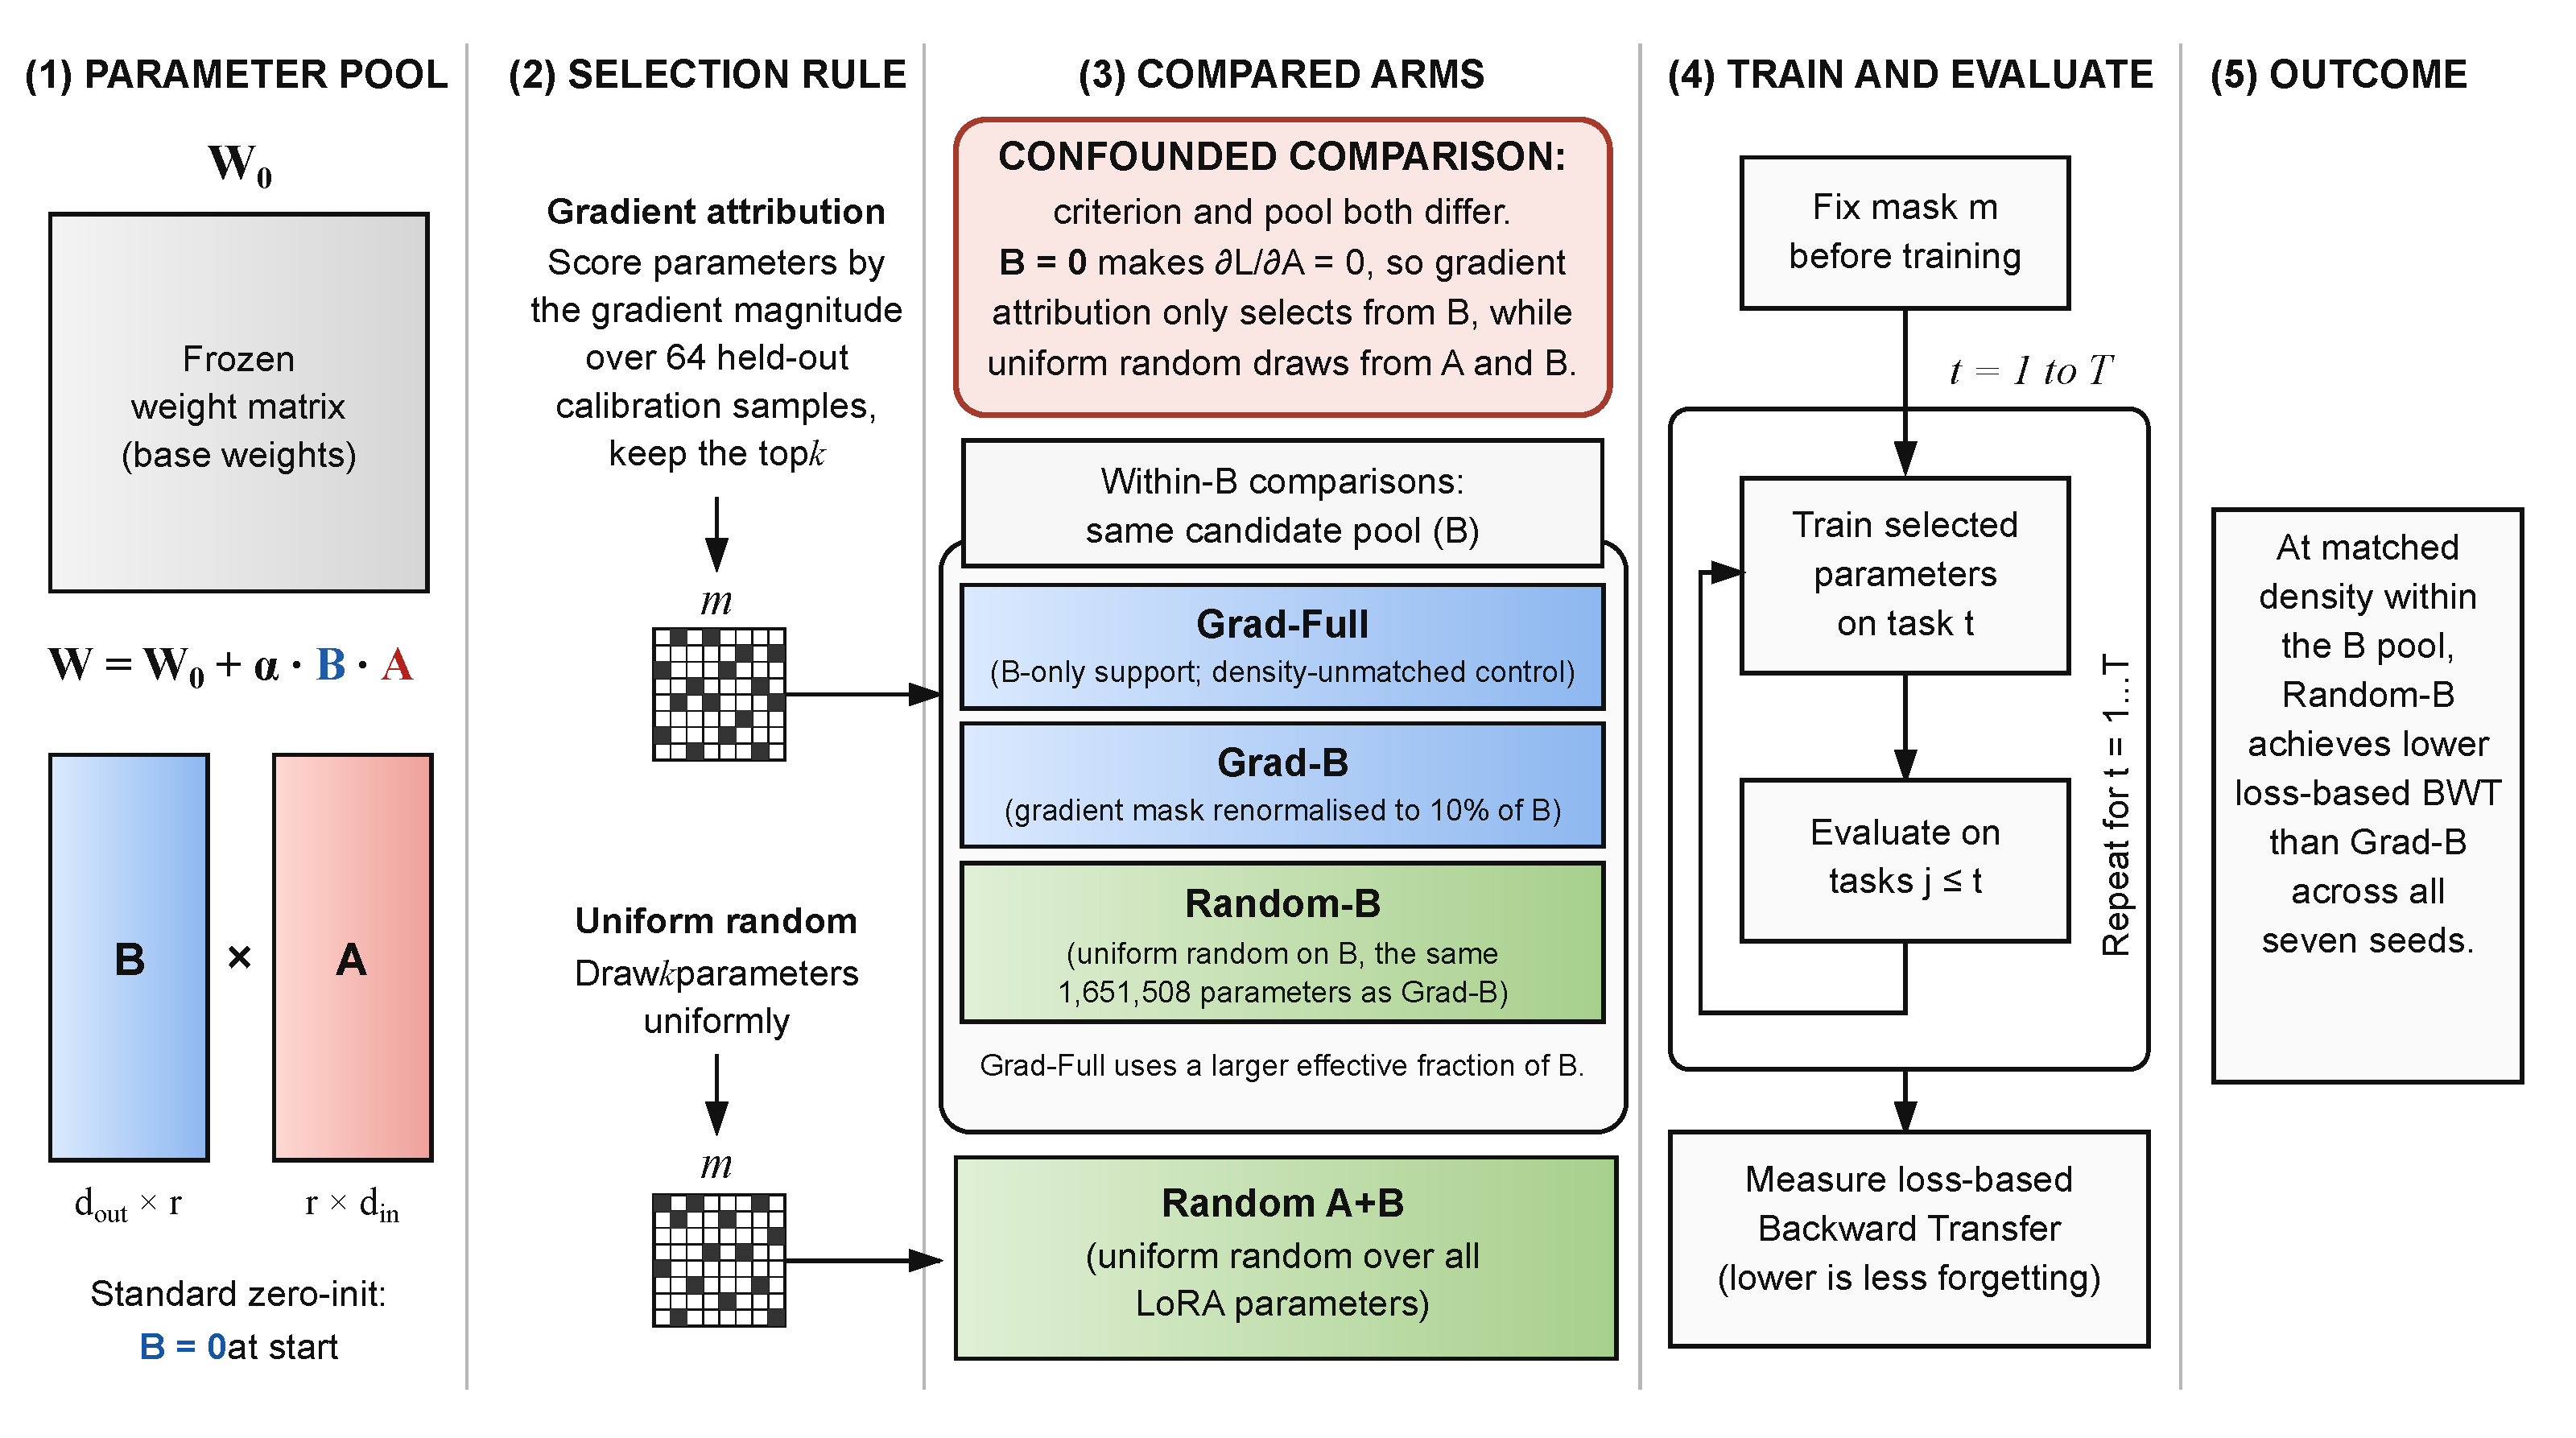
\includegraphics[width=\textwidth]{figures/figure1a_method_overview_corrected_v6.pdf}
\centerline{\footnotesize (a) Method and comparison.}
\end{minipage}\hfill
\begin{minipage}[b]{0.60\textwidth}
\centering
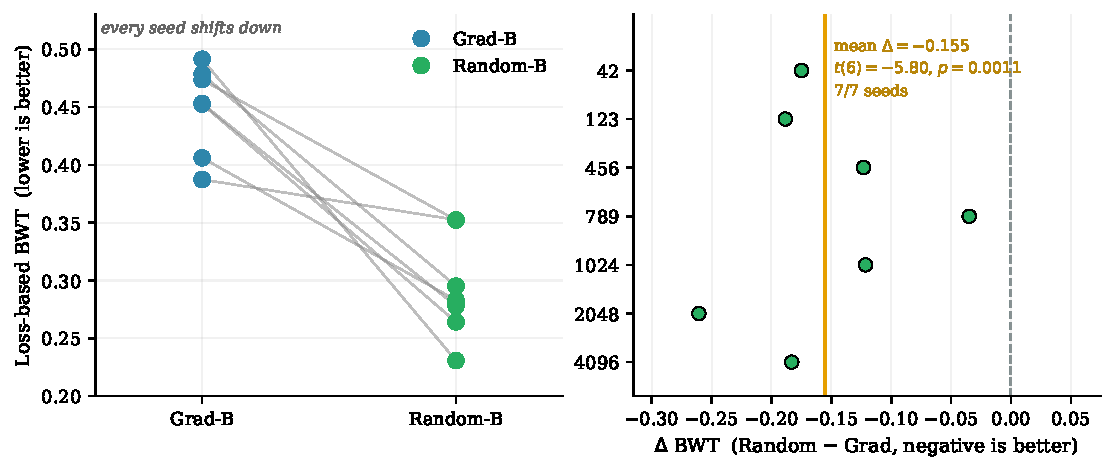
\includegraphics[width=\textwidth]{figures/fig1_main_results.pdf}
\centerline{\footnotesize (b) Key effect (D1, seven seeds).}
\end{minipage}
\caption{The density-matched comparison. (a) Both arms draw 10\% of the rank-16 \texttt{lora\_B} pool, so they train exactly the same 1.6M parameters and differ only in how those coordinates are chosen; because $B=0$ at initialization, the gradient score is zero for every \texttt{lora\_A} coordinate, and any baseline that draws from both pools changes the pool as well as the criterion. (b) Under that matched density the random mask achieves lower loss-based BWT than the gradient mask in all seven seeds. 
% (mean $\Delta = -0.155$, $p = 0.0011$).
}
\label{fig:headline}
\end{figure}



% \paragraph{Contributions.}
% \begin{enumerate}[nosep,leftmargin=*]
% \item 
\textbf{A gradient-attribution confound in LoRA continual learning.} Under zero-init LoRA the gradient with respect to \texttt{lora\_A} is identically zero, so gradient masks select from \texttt{lora\_B} only while the usual random baseline draws from both pools. Comparisons that do not match the pool compare a selection rule against a selection rule plus a pool change.
% \item 
\\
% \textbf{Density-matched evidence that random selection is not worse.} At equal parameter count the random mask achieves the lower loss-based BWT in every seed, an advantage concentrated on the medical task, with code and math in the same direction and no reliable difference on legal. The pattern is a stability--plasticity trade-off, not a uniformly better mask.
% % \item 
% \\
% \textbf{An engineering recommendation: drop the attribution pass.} At matched density a zero-cost random mask is not worse on loss-based forgetting. On the two discrete-option tasks (Medical, Legal), the two masks are statistically indistinguishable, and a 4-percentage-point non-inferiority margin specified in advance is not met: accuracy differences of up to about 4.8 percentage points in the gradient mask's favour are not excluded by this measurement. The recommendation is therefore scoped to the loss evidence, and it removes the per-task backward pass over the calibration set (64 forward--backward steps, 12.8\% on top of the training budget) together with the calibration-set dependency.

% \textbf{Empirical findings under density matching and practical recommendations:} Holding parameter counts strictly equal, uniform random masking matches or beats compute-heavy gradient attribution on loss-based backward transfer, yielding consistently lower forgetting across all seeds due to a favorable stability–plasticity trade-off. On discrete-option task accuracy, the two strategies remain statistically indistinguishable. Based on these loss-based findings, we recommend dropping the calibration attribution pass in continual learning. Doing so eliminates per-task calibration backpropagation (64 forward–backward steps, a 12.8% saving on training compute) and frees the pipeline from calibration dataset dependencies.

\textbf{Density-matched evidence and engineering recommendation.} Under strict equal-parameter control, a zero-cost random mask performs no worse than gradient attribution on loss-based backward transfer (Loss-based BWT), achieving lower forgetting across all seeds—an advantage reflecting a fundamental stability–plasticity trade-off. On task accuracy for discrete-option benchmarks, the two masks are statistically indistinguishable. Backed by the loss evidence, we offer a practical engineering recommendation: drop the attribution pass entirely. This removes the per-task backward overhead over the calibration set (64 forward–backward steps, saving 12.8\% of the training budget) while eliminating dependency on external calibration data.

% \end{enumerate}

% All reported forgetting metrics are loss-based BWT. All headline comparisons are within-run.
